\documentclass[a4paper,12pt]{article} %размер бумаги устанавливаем А4, шрифт 12 пунктов

\usepackage[utf8]{inputenc}%включаем свою кодировку: koi8-r или utf8 в UNIX, cp1251 в Windows
\usepackage[english,russian]{babel}%используем русский и английский языки с переносами
\usepackage{cmap}

\usepackage{amsmath} %подключаем нужные пакеты расширений
\usepackage{graphicx} % Allows including images
\usepackage{url}

\usepackage{geometry} % Меняем поля страницы
\geometry{left=2cm}% левое поле
\geometry{right=1.5cm}% правое поле
\geometry{top=1.5cm}% верхнее поле
\geometry{bottom=1.5cm}% нижнее поле

\usepackage{listings}
\usepackage{xcolor} % for setting colors
\definecolor{sh_comment}{rgb}{0.12, 0.38, 0.18 } %adjusted, in Eclipse: {0.25, 0.42, 0.30 } = #3F6A4D
\definecolor{sh_keyword}{rgb}{0.37, 0.08, 0.25}  % #5F1441
\definecolor{sh_string}{rgb}{0.06, 0.10, 0.98} % #101AF9

\DeclareUnicodeCharacter{00A0}{~}

% set the default code style
\lstset{
    frame=tb, % draw a frame at the top and bottom of the code block
    tabsize=4, % tab space width
    basicstyle=\small,
    showstringspaces=false, % don't mark spaces in strings
    numbers=left, % display line numbers on the left
    stringstyle=\color{sh_string},
    keywordstyle = \color{sh_keyword}\bfseries,
    commentstyle=\color{sh_comment}\itshape % string color
}

\begin{document}


\begin{titlepage}
\newpage

\begin{center}
Санкт-Петербургский государственный политехнический университет \\
Институт Информационных Технологий и Управления \\*
Кафедра компьютерных систем и программных технологий \\*
\hrulefill
\end{center}

\vspace{18em}

\begin{center}
\Large Отчет по расчетной работе № 3 \\ по предмету «Системное программное обеспечение» \\
\end{center}

\vspace{1em}

% \linebreak
\begin{center}
\textsc{\textbf{Примитивы синхронизации в ОС Windows}}
\end{center}

\vspace{16em}

\begin{flushleft}
Работу выполнил студент гр. 53501/3\hrulefill Мартынов С. А. \\
\vspace{1.5em}
Работу принял преподаватель \hrulefill Душутина Е. В. \\
\end{flushleft}

\vspace{\fill}

\begin{center}
Санкт-Петербург \\
2014
\end{center}

\end{titlepage}
\newpage

%------------------------------------------------
\section*{Постановка задачи}

В рамках данной работы необходимо ознакомиться с основными примитивами синхронизации в ОС Windows, и выполнить следующие задачи:
\begin{enumerate}
\item Привести собственные результаты выполнения предложенных программ и их анализ:
\begin{itemize}
\item Использование мьютексов
\item Использование семафоров
\item Критические секции
\item Объекты-события в качестве средства синхронизации
\item Условные переменные
\item Задача читатели и писатели
\item Решение задачи читатели-писатели для потоков
разных процессов с синхронизацией объектами
\end{itemize}
\item Модифицировать предложенное решение таким образом, чтобы читатели не имели доступа к памяти по записи.
\item Предложить более рациональное решение задачи читатели-писатель, используя другие средства синхронизации или их сочетание. Объяснить и подтвердить экспериментально улучшение характеристик взаимодействия.
\item Разработать клиент-серверное приложение для полной задачи читатели-писатели с собственной системой ограничений на доступ каждого читателя к информации.
\item Разработать программу читатели-писатели для сетевого функционирования. Для этого выбрать подходящие средства IPC и синхронизации.
\item Предложить программное решение задачи производители-потребители (разница с предыдущей задачей - возможность модификации считываемых данных).
\item Решить задачу обедающие философы, обосновать выбранные средства синхронизации.
\end{enumerate}

\vspace{1em}
Исходный код всех представленных листингов доступен по адресу \\ \url{https://github.com/SemenMartynov/SPbPU_SystemProgramming}.

\setcounter{page}{2}

\newpage
%------------------------------------------------
\section*{1.1 Использование мьютексов}

\begin{figure}[h!]
\centering
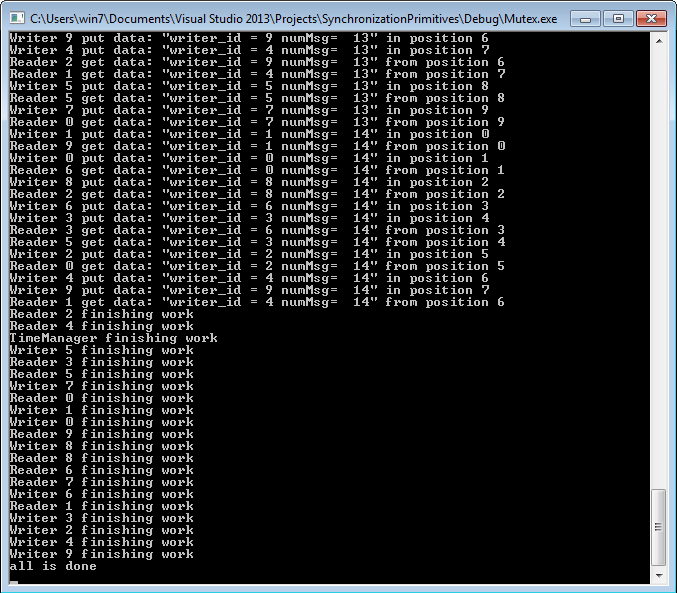
\includegraphics[scale=1]{res/001}
\caption{Использование мьютексов.}
\end{figure}

\newpage

%------------------------------------------------
\section*{1.2 Использование семафоров}

\begin{figure}[h!]
\centering
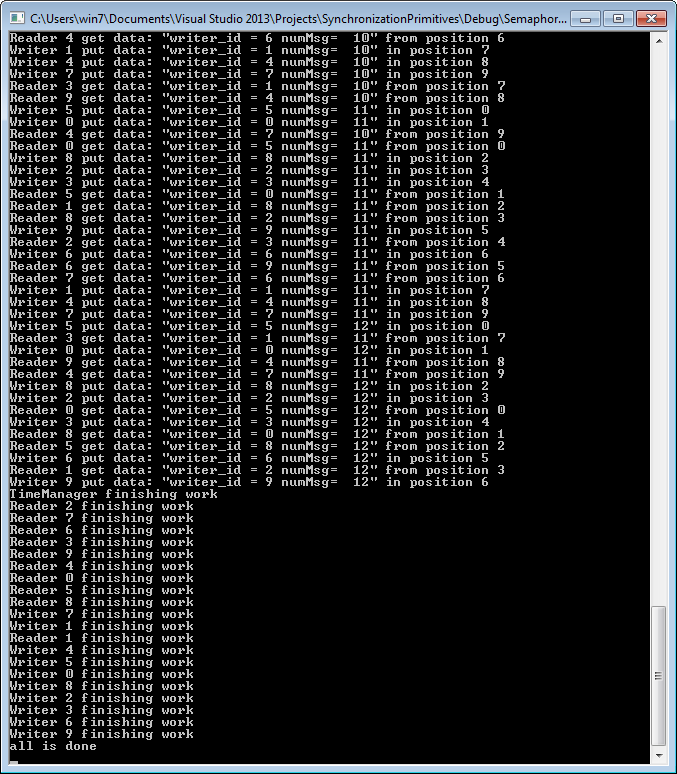
\includegraphics[scale=1]{res/002}
\caption{Использование семафоров.}
\end{figure}

\newpage

%------------------------------------------------
\section*{1.3 Критические секции}

\begin{figure}[h!]
\centering
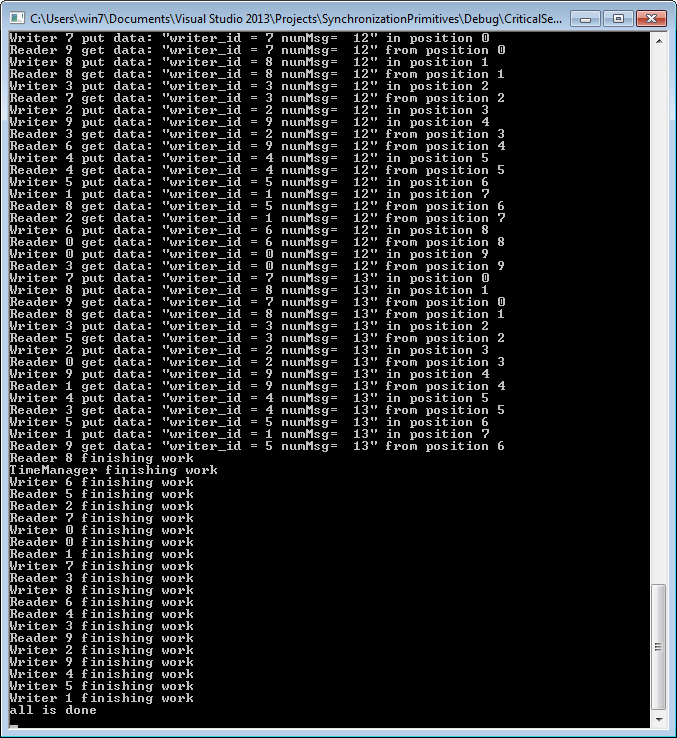
\includegraphics[scale=1]{res/003}
\caption{Критические секции.}
\end{figure}

\newpage

%------------------------------------------------
\section*{1.4 Объекты-события в качестве средства синхронизации}

\begin{figure}[h!]
\centering
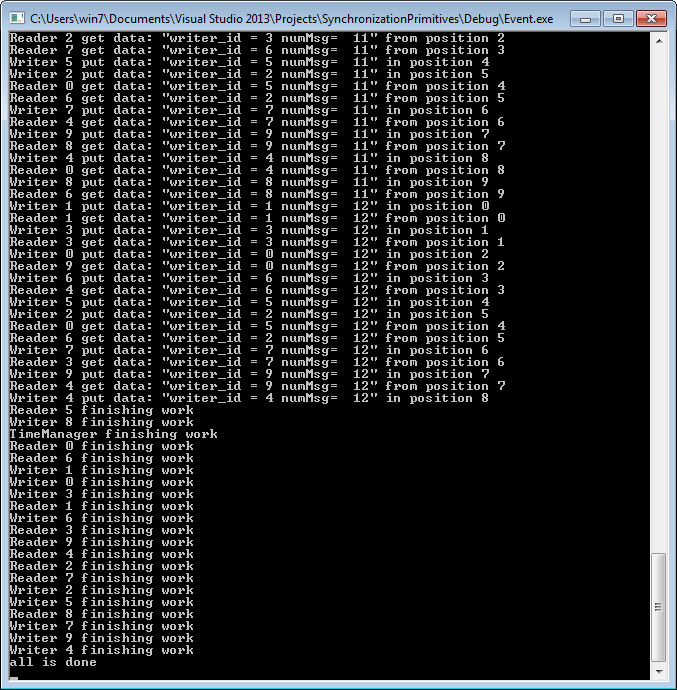
\includegraphics[scale=1]{res/004}
\caption{Объекты-события в качестве средства синхронизации.}
\end{figure}

\newpage

%------------------------------------------------
\section*{1.5 Условные переменные}

\begin{figure}[h!]
\centering
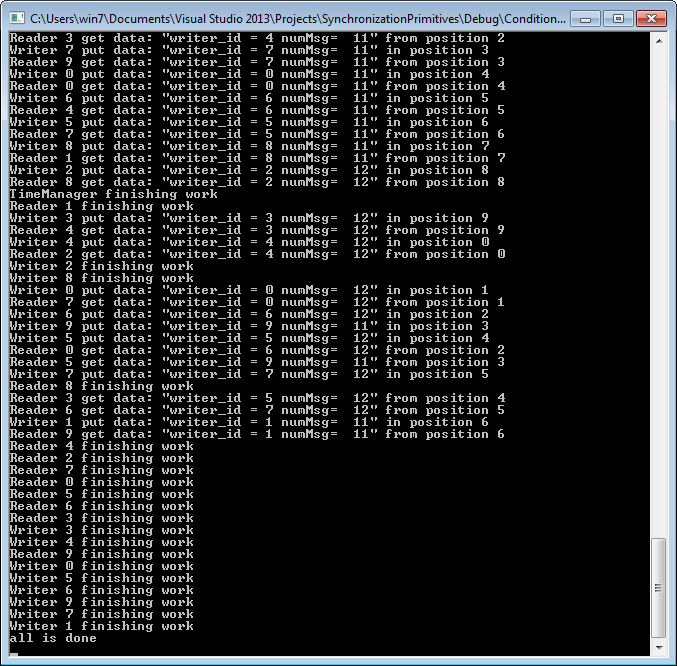
\includegraphics[scale=1]{res/005}
\caption{Условные переменные.}
\end{figure}

\newpage

%------------------------------------------------
\section*{1.6 Задача читатели и писатели}

\begin{figure}[h!]
\centering
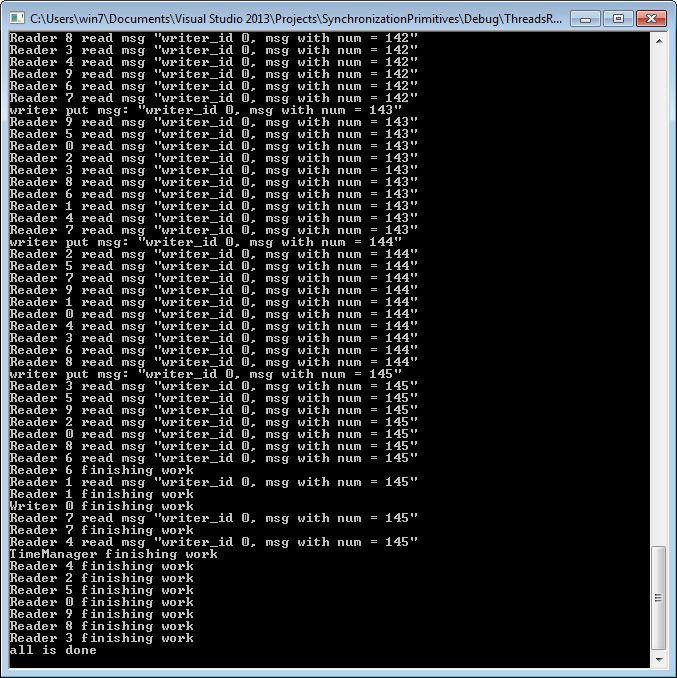
\includegraphics[scale=1]{res/006}
\caption{Задача читатели и писатели.}
\end{figure}

\newpage

%------------------------------------------------
\section*{1.7 Решение задачи читатели-писатели для потоков}

\begin{figure}[h!]
\centering
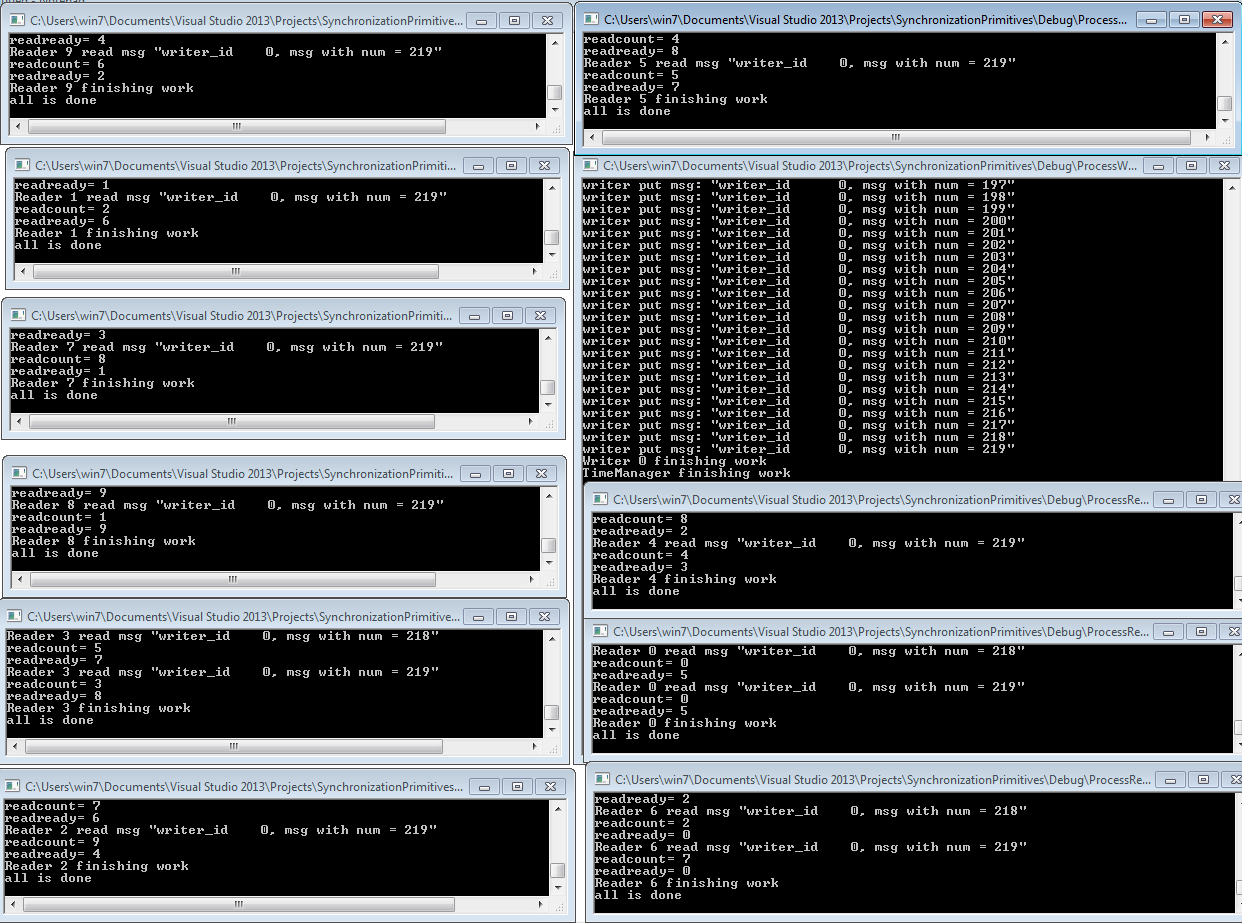
\includegraphics[scale=0.50]{res/007}
\caption{Решение задачи читатели-писатели для потоков.}
\end{figure}

\newpage

%------------------------------------------------
\section*{2 Модификация задачи читатели-писатели без доступа читателей на запись}

\begin{figure}[h!]
\centering
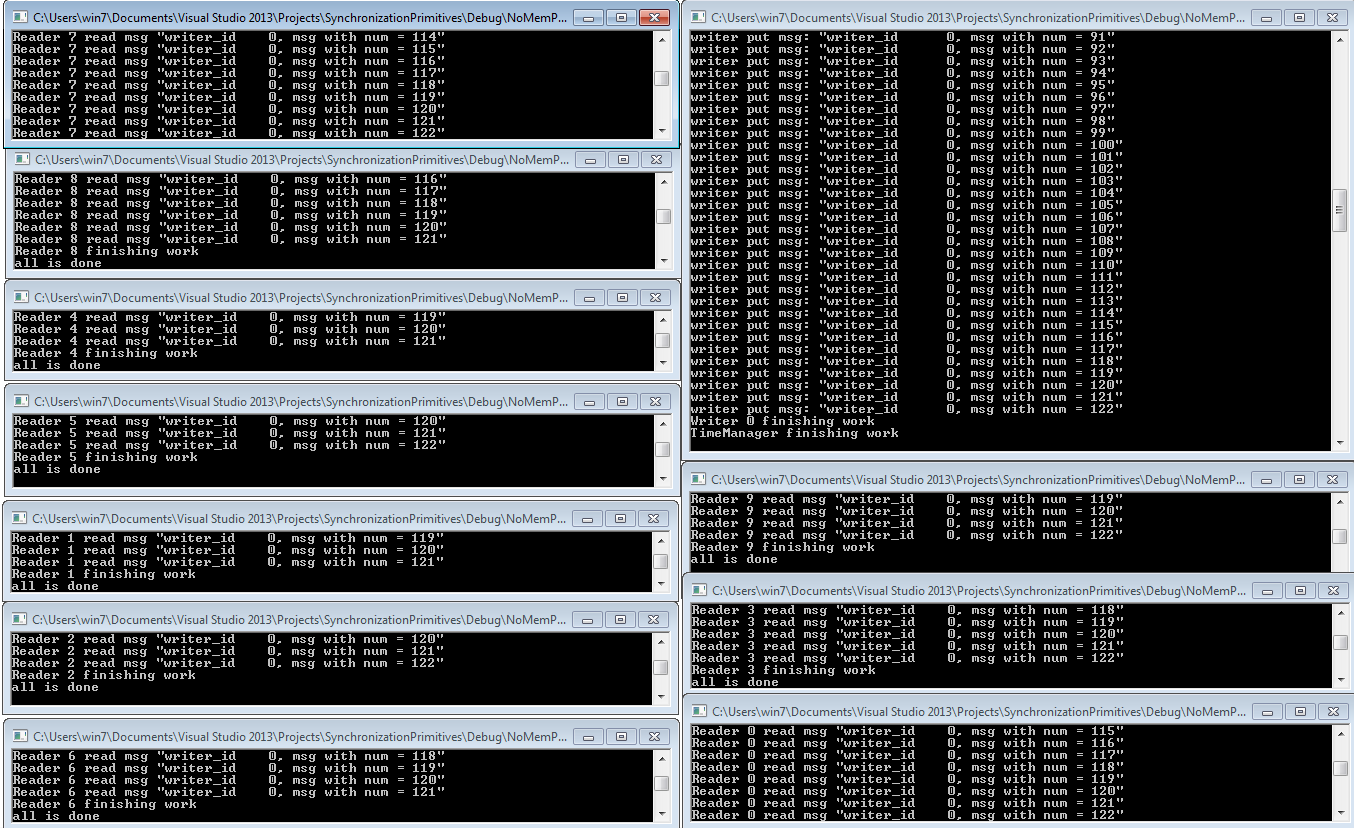
\includegraphics[scale=0.50]{res/008}
\caption{Модификация задачи читатели-писатели.}
\end{figure}

\newpage


%------------------------------------------------
\section*{Выводы}


\end{document}
